\chapter{Entorno Empresarial}

En este capítulo se presenta información relacionada al ambiente de trabajo en el que se realizó la pasantía, con el propósito de que el lector conozca un poco más a la empresa \business desde una breve descripción hasta su organización interna, objetivos y metas.

\section{Descripción de la empresa}

\business es una empresa venezolana fundada en el año 2014, con una propuesta innovadora que busca conectar profesionales independientes que ofrecen variadas actividades con usuarios que deseen hacer algo nuevo, de una manera fácil mediante el uso de la tecnología. Actualmente tiene como meta conectar a las personas a través de actividades y la facilidad de comunicación sobre ellas, tanto si se realizan dentro como fuera de la ciudad.

\section{Visión}

``Usar la tecnología para desprendernos de ella, conectando personas, lugares y experiencias para multiplicar la emoción por descubrir'' \cite{zomoz}.

\section{Misión}

``Ser una plataforma de confianza, fácil de usar, experta en ofrecer actividades y viajes auténticos creados por personas que comparten su estilo de vida haciendo a todos parte de una comunidad transformadora'' \cite{zomoz}

\section{Objetivo}

``Ofrecer las mejores actividades y experiencias en todas las ciudades de América Latina en el corto plazo y en el mundo en el mediano largo plazo'' \cite{zomoz}

\section{Organización}

\business es una empresa pequeña y joven, con pocos departamentos y subdepartamentos. En la figura \ref{fig:organization} se puede observar el organigrama de la empresa.

\begin{figure}
  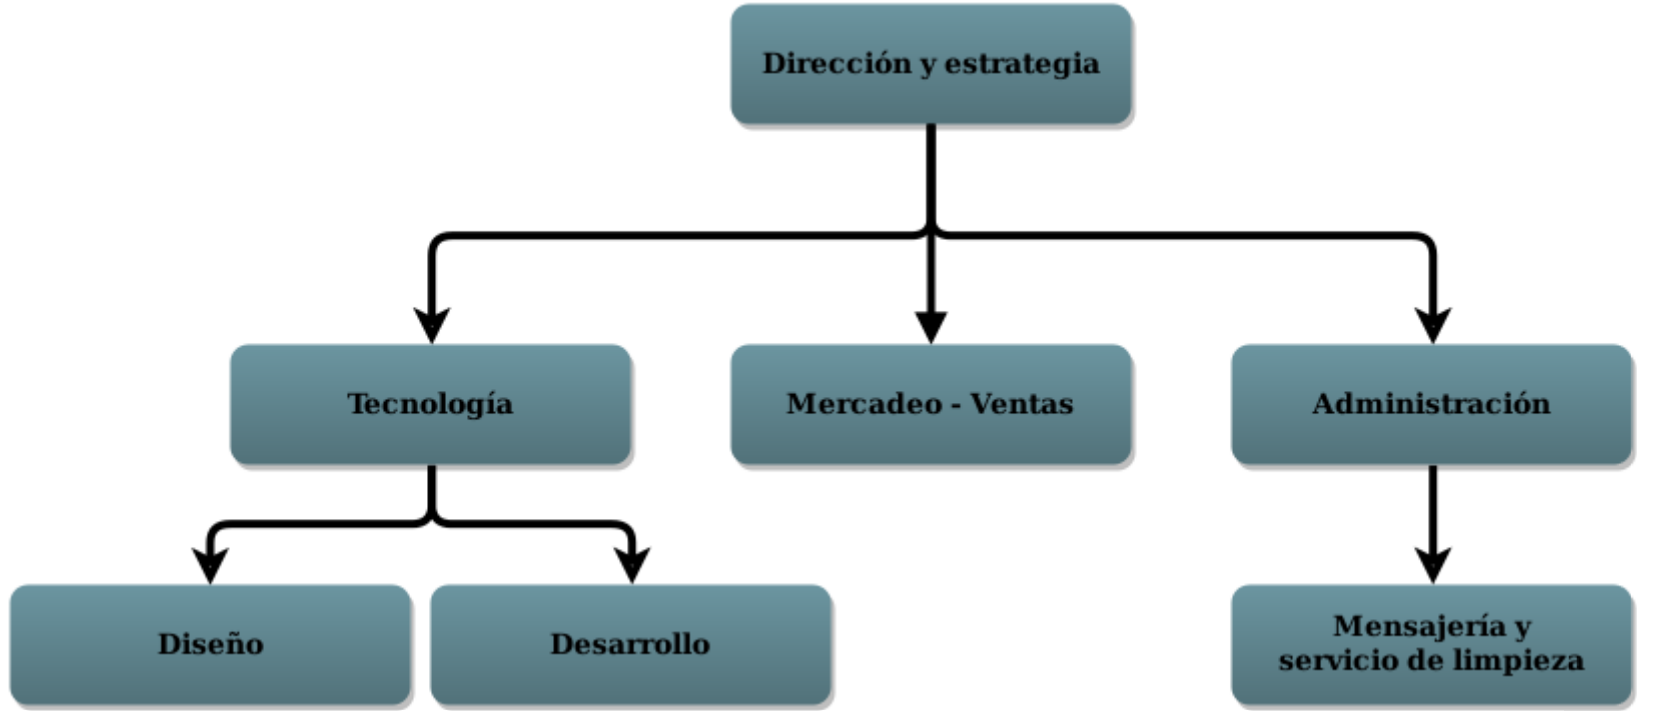
\includegraphics[width=\linewidth]{figures/organization.png}
  \caption{Organigrama de \business}
  \label{fig:organization}
\end{figure}

Los departamentos que conforman a la empresa son:

\begin{itemize}
  \item Dirección y estrategia: Se encarga de la dirección general de la empresa, el establecimiento de las metas para el corto, mediano y largo plazo, además de fijar el camino para cumplirlas.
  \item Tecnología: Se encarga del mantenimiento y mejora constante de los recursos tecnológicos de la empresa.
  \item Diseño: Se encarga del diseño artístico del producto principal de la empresa, así como la identidad visual de la empresa y material gráfico publicitario.
  \item Desarrollo: Se encarga del diseño, desarrollo, implementación y mantenimiento de soluciones tecnológicas usadas en el producto de la empresa, así como otras tareas relacionadas al ámbito tecnológico.
  \item Mercadeo - Ventas: Se encarga del diseño de las campañas de \textit{marketing}, fidelización y atención al cliente, afiliaciones y venta de actividades.
  \item Administración: Se encarga del área administrativa de la empresa, desde contabilidad, finanzas e inventario hasta recursos humanos.
  \item Mensajería y servicio de limpieza: Encargada de la recepción y envíos de encomiendas e higienización del ambiente de trabajo.
\end{itemize}

\section{Ubicación del pasante}

El pasante se ubicó como \textit{Frontend Developer} en el subdepartamento de Desarrollo, bajo la supervisión del Ingeniero Juan Arocha como tutor industrial.
